
\section{Background}
\label{s:background}

\begin{figure}
 \centering
 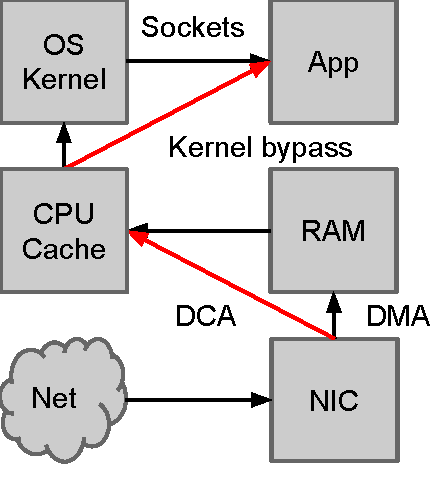
\includegraphics[width=0.5\columnwidth]{figures/net_simple.pdf}
 \caption{Simplified network stack diagram.}
 \label{f:net_stack}
\end{figure}

%High performance network stacks typically avoid unnecessary copying. 
Figure \ref{f:net_stack} shows a high level view of a typical network stack. 
Packets from the network are delivered from the network card into system memory via Direct Memory Access (DMA) or Direct Cache Access (DCA) in high performance cards. 
The Operating System kernel network stack then processes the packet before delivering packet to the application. 
Some high performance systems use kernel bypass to deliver packets directly to a network stack inside of the application which saves on copy costs. 